\chapter{推与拉：力}\label{ch:g2:pushes-and-pulls}

开门、拉拉链、踢球、拖雪橇：你的一整天
都在推和拉。物理学把这些统称为一个了不起的名字
——力——，并提出两个简单的问题：力能做什么，
它朝哪个方向作用？

\section{处处都有推和拉}

\begin{definition}[力]\label{def:g2:pushes-and-pulls:force}
一个\emph{力}\index{力}就是一次推或一次拉。推秋千、
拉小车、按门铃、拉伸橡皮筋、
捏面团：这些都是正在起作用的力。
力总有大小——轻柔还是强劲——还有
\emph{方向}：它朝\emph{某个方向}推或拉。
\end{definition}

\begin{example}[推还是拉？]\label{ex:g2:pushes-and-pulls:sort}
数一数你的一天：踢球，是用脚推。拉开
抽屉，是拉。关上抽屉，是推。拉上外套的拉链，是
拉。揉面团，是许多次小小的推。拔河，是两队人
朝相反方向拉同一根绳子。
\end{example}

\begin{method}[用箭头画力]\label{met:g2:pushes-and-pulls:arrow}
物理学家把力画成一个\emph{箭头}：
\begin{enumerate}
  \item 箭头从推或拉抓住物体的地方开始；
  \item 箭头指向力作用的方向；
  \item 力越大，箭头越长。
\end{enumerate}
一支小小的箭头，就能说清全部情况：在哪里，朝哪边，用了多大的力。
以后还会画很多这样的箭头。
\end{method}

\begin{omfigure}
\begin{tikzpicture}[scale=0.85]
  \draw[thick] (0,0) -- (4.6,0);
  \draw[thick, fill=omMeth, fill opacity=0.4] (1.4,0) rectangle (2.9,1.0);
  \draw[-Stealth, very thick, omThm] (0.2,0.5) -- (1.3,0.5);
  \node[below, font=\small] at (2.3,-0.25) {轻轻一推：箭头短};
  \draw[thick] (6.4,0) -- (11.0,0);
  \draw[thick, fill=omMeth, fill opacity=0.4] (8.4,0) rectangle (9.9,1.0);
  \draw[-Stealth, very thick, omThm] (6.5,0.5) -- (8.3,0.5);
  \node[below, font=\small] at (8.7,-0.25) {用力一推：箭头长};
\end{tikzpicture}

{\small 同一个箱子被推了两次。箭头表示推在哪里，
朝哪个方向作用，还有用了多大的力——由箭头的长短来表示。}
\end{omfigure}

\begin{omfigure}
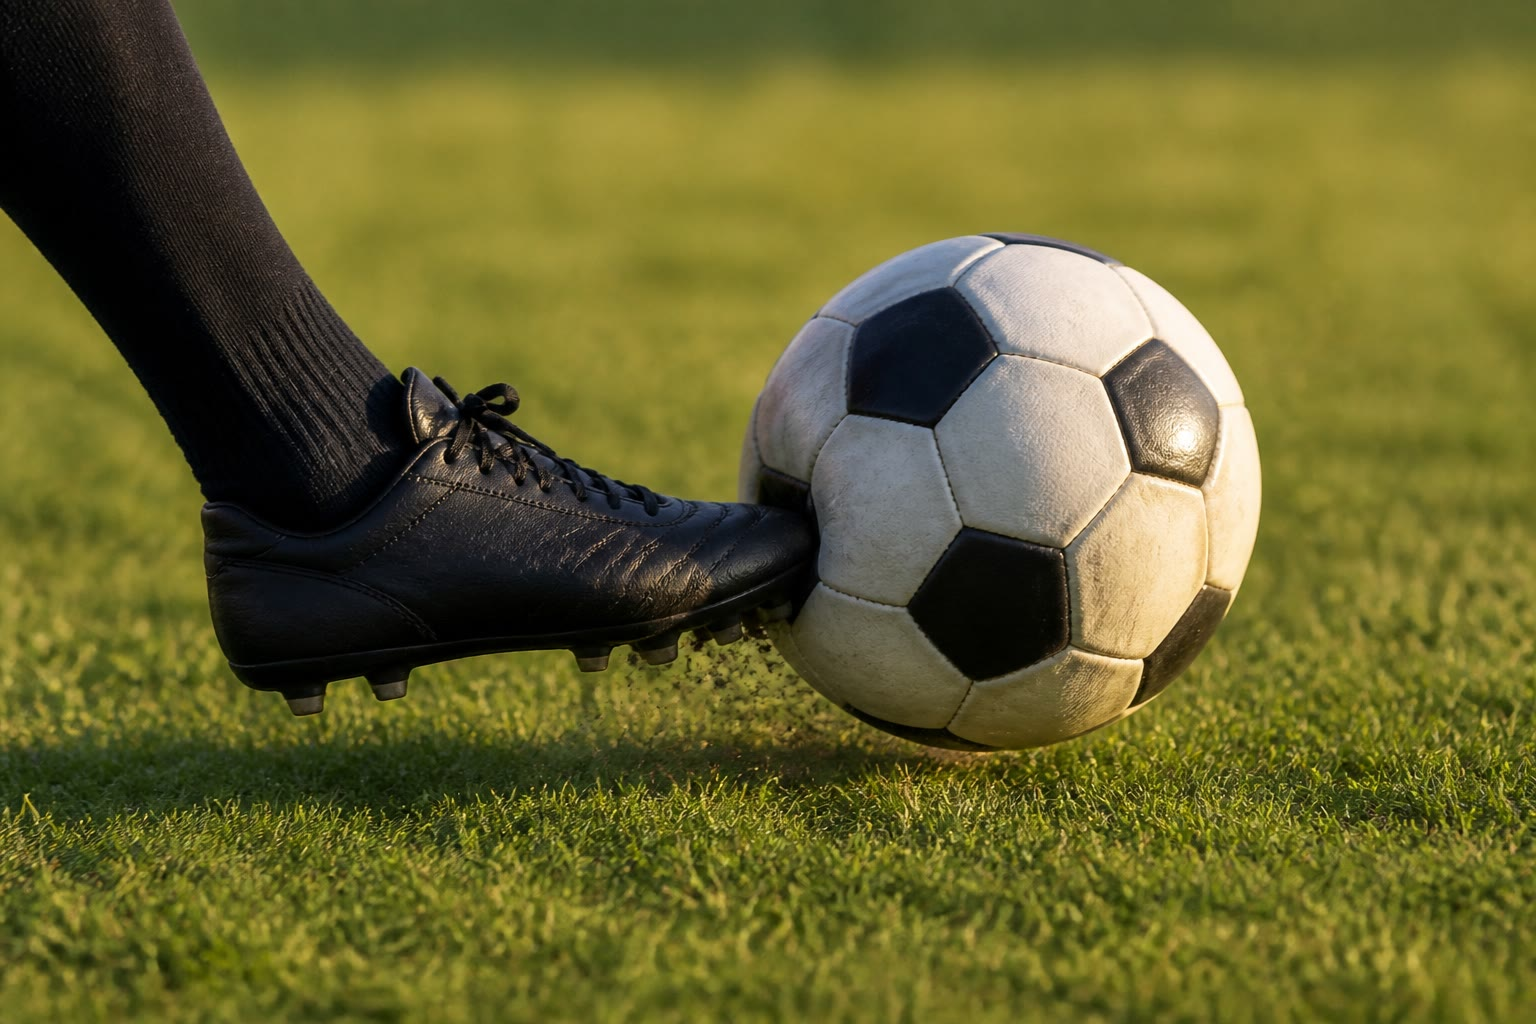
\includegraphics[width=0.58\linewidth]{images/book1/ai/g2-pushes-kick.jpg}

{\small 力作用的那一刻：靴子在推，静止的球就要飞出去。}
\end{omfigure}

\section{力能做什么}

\begin{proposition}[力的四种作用]\label{prop:g2:pushes-and-pulls:jobs}
力可以对物体做四件事：
\begin{enumerate}
  \item 使它\emph{开始}运动——
        一脚踢出，静止的球飞走了；
  \item 使它\emph{停下}——守门员的手挡住了射门的球；
  \item 使它\emph{转向}——侧面轻轻一拨，滚动的球的
        路线就弯了；
  \item 使它\emph{改变形状}——挤压使海绵变扁，
        拉伸使橡皮筋变长。
\end{enumerate}
没有力，就没有这四种作用：一个完全不受外力的物体，
会一直保持原来的状态。
\end{proposition}

\begin{omfigure}
\begin{tikzpicture}[scale=0.85]
  \draw[dashed, omExo] (0,0.6) -- (4.2,0.6);
  \fill[omDef] (0.6,0.6) circle (0.24);
  \fill[omDef, opacity=0.45] (3.0,0.6) circle (0.24);
  \draw[-Stealth, very thick, omThm] (4.2,0.6) -- (6.0,1.7);
  \fill[omDef, opacity=0.45] (5.4,1.33) circle (0.24);
  \draw[-Stealth, thick, omThm] (4.2,-0.35) -- (4.2,0.5);
  \node[below, font=\small, omThm] at (4.2,-0.5) {此处侧面轻拨};
  \node[below, font=\small] at (1.4,0.3) {沿直线滚动};
  \node[right, font=\small] at (5.85,2.05) {方向变了！};
\end{tikzpicture}

{\small 第三种作用：滚动的球受到侧面的轻拨，
路线朝着推的方向弯了。}
\end{omfigure}

\begin{example}[力越强，效果越大]\label{ex:g2:pushes-and-pulls:stronger}
轻轻拨一下弹珠，它慢慢滚到桌子边缘。用力弹
出去，它就飞过整个房间。同一颗弹珠，同一根
手指——只是推的力变了，弹珠的飞行也随之改变。
力轻，效果就轻；力大，效果就大。
\end{example}

\begin{example}[动手试一试：形状的变化]\label{ex:g2:pushes-and-pulls:shape}
找来一块海绵、一根橡皮筋、一团橡皮泥和一块木块。
分别挤一挤、拉一拉。松手的那一刻，海绵会
弹回原来的样子；橡皮筋也一样。橡皮泥会保持
新的形状——你的力在上面留下了永久的凹痕。那木块呢？你最用力的挤压，
也没有让它有任何变化（至少你看不出来！）。各种物体对力的反应，
各有各的方式。
\end{example}

\section{不接触的力}

\begin{example}[地球的拉力]\label{ex:g2:pushes-and-pulls:earthpull}
松手让勺子掉下去：它会往下落。把球抛得再高，
它终究会落回来。树叶、雨滴、碎屑——凡是松手的东西，
都会\emph{向下}落。总有一种力在时时刻刻拉着它们，
却并不与它们接触：这就是地球本身。地球的拉力
是你生活中最稳定的力——它从不松手，也正因为如此，
操场上的“下”在任何地方都是同一个方向。
\end{example}

\begin{omfigure}
\begin{tikzpicture}[scale=0.85]
  % the falling apple
  \draw[thick] (0,0) -- (5.0,0);
  \draw[thick, red!60!black, fill=red!70] (1.4,2.5) circle (0.32);
  \draw[thick, brown!60!black]
    (1.4,2.82) .. controls (1.45,2.98) .. (1.56,3.08);
  \draw[thick, green!45!black, fill=green!45]
    (1.62,3.02) ellipse [x radius=0.16, y radius=0.07, rotate=30];
  \draw[-Stealth, very thick, omDef] (1.4,2.05) -- (1.4,1.1);
  \node[right, font=\small, omDef] at (1.65,1.6)
    {地球向下拉};
  \node[below, font=\small] at (2.5,-0.25)
    {苹果下落：被拉，而不是被推};
  % the magnet holding a paperclip up across a gap
  \draw[thick, fill=red!70] (7.9,2.35) rectangle (8.75,2.95);
  \draw[thick, fill=blue!60] (8.75,2.35) rectangle (9.6,2.95);
  \begin{scope}[shift={(8.54,1.65)}, rotate=-90]
    \draw[thick, rounded corners=2.6pt]
      (0,0) -- (1.1,0) -- (1.1,0.42) -- (0.12,0.42) -- (0.12,0.14)
      -- (0.95,0.14) -- (0.95,0.30) -- (0.30,0.30);
  \end{scope}
  \draw[-Stealth, very thick, omDef] (9.15,1.0) -- (9.15,2.0);
  \node[below, font=\small] at (8.75,0.1)
    {磁铁向上拉 --- 不接触};
\end{tikzpicture}

{\small 两种不接触的力：地球隔着空气把苹果向下拉；
磁铁隔着空气把回形针向上拉。}
\end{omfigure}

\begin{remark}[老朋友]\label{rem:g2:pushes-and-pulls:magnets}
你已经认识了另一种不接触的力：磁铁，它能隔着空气
吸住回形针。磁铁和地球的拉力是你日常生活中
少有而珍贵的两种不接触的力——
是例外，因为你遇到的其他推或拉都需要接触。
这两种力在本课程后面都会展开为重要的章节。
\end{remark}

\section{练习}

\begin{exercise}[$\star$]\label{exo:g2:pushes-and-pulls:1}
推还是拉？按门铃；\ 拉开抽屉；\ 用头顶
足球；\ 拖着雪橇上坡；\ 挤牙膏。
\end{exercise}

\begin{exercise}[$\star$]\label{exo:g2:pushes-and-pulls:2}
力的箭头能告诉我们力的哪三件事？
\end{exercise}

\begin{exercise}[$\star$]\label{exo:g2:pushes-and-pulls:3}
说出力的四种作用，并为每一种举一个自己的例子 ---
与本章中的例子不同。
\end{exercise}

\begin{exercise}[$\star$]\label{exo:g2:pushes-and-pulls:4}
一颗弹珠笔直地朝你滚来。只用一根手指，
你怎样让它：停下？\ 加速？\ 偏向一旁？每次都说出
手指朝哪个方向推。
\end{exercise}

\begin{exercise}[$\star$]\label{exo:g2:pushes-and-pulls:5}
哪些会弹回，哪些会保留凹痕：海绵；\
橡皮泥；\ 橡皮筋；\ 松软的雪？
\end{exercise}

\begin{exercise}[$\star$]\label{exo:g2:pushes-and-pulls:6}
画出一个箱子被轻轻地向右推，再画出同一个箱子被
用力地向左推。两个箭头有什么不同？
\end{exercise}

\begin{exercise}[$\star$]\label{exo:g2:pushes-and-pulls:7}
什么力使每一样被松开的东西都会下落？它需要接触
正在下落的勺子吗？它总是朝哪个方向拉？
\end{exercise}

\begin{exercise}[$\star$]\label{exo:g2:pushes-and-pulls:8}
说出你已经认识的两种不接触的力，每种都举一个
在家里见到的例子。
\end{exercise}

\begin{exercise}[$\star\star$]\label{exo:g2:pushes-and-pulls:9}
在拔河比赛中，两队都用尽全力拉，但绳上的
彩带有时一动也不动。画出绳子，并画出两队的
箭头。两个拉力须满足什么条件，彩带才会
静止不动？一队刚一用力，
拉得更猛时会发生什么？
\end{exercise}

\begin{exercise}[$\star\star$]\label{exo:g2:pushes-and-pulls:10}
一个竖直向上抛出的球，速度变慢，瞬间停住，
再落回来。上升途中、最高点和下落途中，哪个力在起作用？
它会停止拉吗？（在这三个
时刻各画出一个箭头。）
\end{exercise}
